% !TeX program = xelatex
% 2026 CUMCM 电子版论文示例：电子版第一页必须是摘要专用页。
% 编译：latexmk -xelatex cumcm.tex
\documentclass[zihao=-4,a4paper,UTF8,fontset=none]{ctexart}

% template
\usepackage{cumcm2026}

% 问题二正文所需的数学、表格与浮动体支持
\usepackage{amsmath,amssymb,amsthm,booktabs,array,graphicx,float,needspace,longtable}
\usepackage{tikz,pgfplots}
\usetikzlibrary{calc,arrows.meta,patterns,positioning}
\pgfplotsset{compat=1.18}
\usepgfplotslibrary{fillbetween}

% 问题二 TikZ 图统一配色
\definecolor{qRedDark}{HTML}{A50026}
\definecolor{qRed}{HTML}{D73027}
\definecolor{qOrange}{HTML}{F46D43}
\definecolor{qOrangeLight}{HTML}{FDAE61}
\definecolor{qYellow}{HTML}{FEE090}
\definecolor{qCyanLight}{HTML}{E0F3F8}
\definecolor{qBlueLight}{HTML}{ABD9E9}
\definecolor{qBlue}{HTML}{74ADD1}
\definecolor{qBlueDark}{HTML}{4575B4}
\definecolor{qNavy}{HTML}{313695}

% 设置一级标题为中文“一、二、三”格式
\ctexset{
  section = {
    number = \chinese{section},
    name = {,、} % 在数字后面加顿号，显示为“一、”
  }
}

% set English and Number font
\setmainfont{TimesNewRoman.ttf}[
  Path=fonts/,
  BoldFont=TimesNewRomanBold.ttf,
  ItalicFont=TimesNewRomanItalic.ttf,
  BoldItalicFont=TimesNewRomanBoldItalic.ttf
]



% set Chinese font
\setCJKmainfont[
  Path=fonts/,
  BoldFont=SimHei.ttf
]{SimSun.ttc}

\setCJKfamilyfont{zhsong}[
  Path=fonts/
]{SimSun.ttc}

\setCJKfamilyfont{zhhei}[
  Path=fonts/,
  BoldFont=SimHei.ttf
]{SimHei.ttf}

% 供 \\texttt、\\path 等等宽环境使用
\setCJKmonofont[
  Path=fonts/,
  BoldFont=SimHei.ttf
]{SimSun.ttc}

\providecommand{\songti}{}
\providecommand{\heiti}{}
\renewcommand{\songti}{\CJKfamily{zhsong}}
\renewcommand{\heiti}{\CJKfamily{zhhei}}





%--------------------------------------------------------------------
%--------------------------------------------------------------------
%以上不要动
%标题与关键词（代码很特殊的写在document环境之前）
\providecommand{\vect}[1]{\boldsymbol{#1}}
\title{题目记得改}
\newcommand{\keywords}{关键词1；关键词2}

\begin{document}

% 2026 电子提交版不得包含承诺书和编号专用页；第一页直接为摘要页。
\maketitle

\begin{cumcmabstract}
针对突发事件中需求不确定、道路通行能力动态变化和多配送中心协同困难的问题，本文构建兼顾响应时间、运输成本与服务公平性的多目标应急物资调度模型。

首先，对需求、库存和路网数据进行一致性校验与异常值处理，并用区间参数描述需求波动。其次，将车辆容量、物资守恒、时间窗和道路容量写入约束，以加权切比雪夫方法获得帕累托折中解。再次，通过滚动时域策略更新需求预测和路径决策。算例结果表明，该方法能够在满足关键需求点最低保障率的同时控制总成本；敏感性分析用于识别需求波动和道路容量对方案稳定性的影响。

最后，从数据误差、参数扰动和极端情景三个层面检验模型，并讨论模型的适用边界。本文方法可为同类多源供给、动态需求的资源配置问题提供可复用的决策框架。

\cumcmkeywords{\keywords}
\end{cumcmabstract}


\section{问题重述}

\subsection{问题背景}

无线电频谱是通信、导航和公共安全等业务稳定运行的重要基础。一旦出现非授权或异常发射信号，相关设备可能受到干扰，进而影响局部区域的无线业务秩序。对干扰源进行处置的关键，在于从广阔区域中快速锁定信号来源，并在确认位置后及时消除干扰。

现有现场处置方式主要依靠人员携带测向设备逐点巡查。该过程需要根据不同地点获得的信号方向信息不断修正判断，既受到仪器读数误差和有效接收范围的限制，也会因人员移动、设备操作和目标确认而消耗较多时间。在存在环境风险或需要快速恢复无线业务的场景中，完全依赖人工排查难以兼顾处置效率与作业安全。

为实现无人化处置，现考虑由机器狗携带测向机、光学探测仪及激光清除装置进入目标区域执行任务。机器狗能够按频道接收信号、在停靠点获取示向度，并在接近目标后完成精确确认和清除。然而，干扰源数目、位置、信号覆盖范围及部分发射方向均未知；同时，测向结果存在有界误差，且移动、频道切换、检测和清除均具有时间代价。因此，需依据有限且带误差的观测信息，构建可靠的定位判据与行动策略，在保证干扰源被清除的前提下尽量缩短总处置时间。

\subsection{问题概述}

\subsubsection{问题一}

针对同一干扰源，已知多个检测点的平面坐标及该干扰源在各检测点处对应的示向度。由于每次示向度读数与真实方向之间存在不超过 $1^\circ$ 的偏差，每个检测结果均对应一个具有角度容差的可能方向范围；多个检测结果共同限定干扰源的可行定位区域。

需要依据给定检测信息，设计计算该定位区域直径的算法，其中直径定义为区域内任意两点距离的最大值；进而讨论直径与该区域相同的圆能否完整覆盖该定位区域。该问题旨在建立测向误差条件下定位不确定性的几何度量，为后续检测点选择提供基础。

\subsubsection{问题二}

已知某全向干扰源在一个检测点处的示向度，现需为机器狗确定第二个检测点。第二次检测应与首次检测形成有效的交会关系，使带误差的两组方向信息能够尽可能缩小干扰源的可能位置范围；同时，所选位置还应满足目标区域及信号有效接收条件，具有实际可达性。

需要给出第二检测点的选择原则，并确定相应的候选区域，以提高后续交会定位的稳定性和精度。

\subsubsection{问题三}

目标圆域内分布有 $10$--$16$ 个全向干扰源，具体数量未知，且各干扰源对应的频道互不相同。机器狗从原点出发，测向机初始频道为 $1$，需自主完成多频道搜索、目标定位和干扰源清除。干扰源的有效接收半径介于 $1000\,\mathrm{m}$ 与 $1500\,\mathrm{m}$ 之间；机器狗移动时不能检测信号，停靠检测时还需计入频道切换和示向度获取时间，接近干扰源后方可借助光学探测仪完成精确定位与清除。

需要构建机器狗在未知多源环境下的搜索、定位、行动决策及清除策略，在确保全部干扰源被清除的前提下最小化定位清除总时间。随后，利用模拟器进行演练测试，并完成三次正式测试，按要求统计每次测试的案例编码、清除干扰源个数、平均定位清除时间及程序运行时间，同时提交对应日志文件。

\subsubsection{问题四}

在问题三的条件下，目标区域内进一步混有全向干扰源和定向干扰源，干扰源总数仍为 $10$--$16$ 个，但各类干扰源数目及定向干扰源的发射方向均未知。定向干扰源仅在其定向方向两侧各 $90^\circ$ 的扇形范围内具有有效辐射，因此，某一检测点未接收到指定频道信号，既可能表示该频道不存在干扰源，也可能意味着该点位于定向干扰源的信号覆盖范围之外。

需要在此条件下重新设计检测、确认与清除策略，使机器狗能够辨别由定向辐射造成的观测缺失，避免遗漏干扰源，并在保证清除完整性的基础上控制总任务时间。通过演练测试和三次正式测试检验策略的有效性，按规定给出测试结果并提交相应日志文件。


\section{问题分析}
将每个子问题拆解为数据、决策变量、约束、目标和验证方式，并说明各子问题之间的数据流与逻辑关系。
\subsection{问题一分析}

问题一要求依据检测点坐标、示向度及其 $\pm1^\circ$ 的误差界，确定定位区域的尺度，并判断以区域直径为直径的圆能否覆盖该区域。分析重点在于将测向约束转化为可计算的几何对象，并区分区域直径与圆覆盖半径的含义。

首先，示向误差具有明确界限，适合采用可行集合描述干扰源的候选位置。单次观测对应误差角域总宽度为 $2^\circ$ 的闭楔形，多次观测通过角域求交形成定位区域。本问围绕示向约束确定的区域展开，目标圆域和有效接收距离等物理约束留待后续搜索问题叠加。

其次，区域尺度的计算需要兼顾正常与退化构型。应先判断观测是否相容、交集是否有界，再区分单点、线段和凸多边形。对于非空有界多边形，可利用半平面交提取顶点，将连续区域上的最远距离问题转化为有限点对搜索，并通过不同实现交叉核验。

最后，最大点对距离与覆盖整个区域所需的半径描述不同的几何性质，不能直接等同。圆覆盖分析需明确直径端点、候选圆心及其余顶点之间的位置关系，建立可计算的覆盖判据；再结合最小覆盖圆与代表性构型，对固定圆心和允许调整圆心两种情形进行比较。
\subsection{问题二分析}

整个问题可以理解为三步：\textbf{第一步：根据第一次测向圈出一条可能范围，第二步：从另一处测向截出较小的重叠区域，第三步：比较不同站位下这块区域有多大。}困难在于，选择第二测点时，真实源点还没有确定。因此，既要让两次测向范围形成交集，不能走到某些点的接收范围之外。

首测示向将源点限制在一个扇形窄角域内，接收半径上界限定源点与首测点的距离。当第二检测点 $q$ 与首测点 $S_1$ 过于接近时，两次观测形成的基线较短。对于 $K_1$ 中的大多数可能源点，两次示向方向近似平行，交会角较小；在 $\pm1^\circ$ 示向误差作用下，两角域的交集会沿纵向明显延伸，导致定位区域直径较大，第二次测向对降低位置不确定性的作用有限。在移动方向合理的前提下，适当增大基线通常能够增大交会角、缩小定位区域，但基线并非越长越好：第二检测点移动过远，可能使部分源点与其距离超过 $1000\,\mathrm{m}$，从而无法接收到信号；移动位置不当还可能进入 $5\,\mathrm{m}$ 近距排除范围，并增加行程时间。因此，第二检测点的选择实质上是一个带探测约束的鲁棒极小极大优化问题，即在保证对任意 $G\in K_1$ 均满足探测条件的前提下，寻找使有界示向误差下最坏定位区域直径最小的测点位置。

题目给出的是示向误差范围，并未指定概率分布。本文首先采用无需分布假设的集合方法：由首测信息构造可行源集，以区域直径表征不确定性，建立保守布点模型。随后通过数值搜索得到推荐点，以全源集扫描检查其最坏表现。最后，在增加概率假设的前提下，额外分析平均精度与尾部风险。

\subsection{问题三分析}

\subsection{问题四分析}

问题四在问题三多频道搜索与清除任务的基础上加入了定向辐射机制。对全向源而言，检测点没有收到信号通常可以用距离超过有效接收半径解释；但对定向源而言，即使检测点与源点距离较近，只要位于其背向半平面内，同样会得到无信号反馈。因此，单次无信号观测不能直接排除检测点附近存在干扰源，也不能据此判定该频道为空。问题的关键由全向情形下的空间覆盖转化为位置、作用半径、源类型和发射朝向的联合不确定性管理。

为兼顾清除可靠性与运行效率，本文采用双层信念描述。第一层仅利用正测向及题设物理边界构造干扰源位置的保守外包区域，用于判断清除点是否具有几何保证；第二层同时利用无信号信息，对位置、作用半径、源类型和朝向进行粒子近似，用于评价下一检测点的发现概率。概率近似只改变探点及访问顺序，不删除第一层的保守区域，因而不会因粒子离散误差破坏清除兜底逻辑。

在策略上，首先以中心及分散检测点完成初始普查；随后将已发现源的候选清除点与未知频道的后验补查点共同纳入路径规划。在每次到达清除位置后，利用该位置对仍未知的频道进行顺路扫描，使清除终点同时成为新的观测站，形成“发现--定位--清除--再发现”的级联过程。最后，依据未知频道仍含活动源的后验风险决定是否增加外圈补查；达到题设源数上限或接近运行时限时终止新增搜索动作。

\subsection{总体思路}
本文先完成数据质量检查，再建立静态基准模型，随后加入不确定性与动态更新机制，最后通过基准对比、敏感性分析和极端情景测试检验结论。
建议来个总体流程图

\section{模型假设}
\noindent 1) 赛题给出的原始数据真实有效；对缺失值和异常值的处理方法在正文中明确说明。

\noindent 2) 单个决策周期内车辆平均速度保持不变；跨周期变化由滚动更新刻画。

\noindent 3) 未显式建模的次要因素对核心结论不产生方向性改变。

\section{符号说明}
表格采用三线表。较长说明列使用自动换行的居中列类型 \texttt{Y}；数值列可使用自动换行的右对齐列类型 \texttt{R}。

\begin{table}[H]
  \centering
  \caption{主要符号与定义}
  \label{tab:symbols}
  \begin{tabularx}{0.86\textwidth}{C{0.18\textwidth}Y R}
    \toprule
    符号 & 含义 & 单位 \\
    \midrule
    $x_{ijk}$ & 车辆 $k$ 是否由节点 $i$ 行驶至节点 $j$ & -- \\
    $q_{ij}$  & 配送中心 $i$ 向需求点 $j$ 配送的物资量 & \si{\kilogram} \\
    $t_j$     & 需求点 $j$ 的实际到达时间 & \si{\minute} \\
    \bottomrule
  \end{tabularx}
\end{table}

\section{模型建立与求解}


\subsection{问题一：交会定位区域的直径与圆覆盖判定}

问题一需要回答两个问题：如何由示向观测计算定位区域的直径，以及以区域直径为直径的圆是否覆盖该区域。题设给出示向误差界而未规定其概率分布，因此先以角域交集描述全部可能位置，再利用凸性将连续区域上的计算转化为有限顶点上的计算。对非空有界凸多边形，取达到最大距离的一对顶点，其连线为一条区域直径，但以该线段为直径的圆不一定覆盖整个区域；覆盖与否可由逐顶点的点积判据确定。

\subsubsection{有界示向误差下的定位区域}

设第 $i$ 个检测点为 $S_i=(x_i,y_i)$，测得示向度为 $\theta_i$，误差上界为 $\varepsilon=\pi/180$。取 $u(\alpha)=(\cos\alpha,\sin\alpha)$，并记二维叉积为 $a\times b=a_xb_y-a_yb_x$。所有角度均按模 $2\pi$ 处理，第 $i$ 次观测确定的闭楔形为
\begin{equation}
W_i=\left\{p\in\mathbb R^2:
\begin{aligned}
&u(\theta_i-\varepsilon)\times(p-S_i)\ge0,\\
&u(\theta_i+\varepsilon)\times(p-S_i)\le0
\end{aligned}\right\}.
\label{eq:q1_wedge}
\end{equation}
两个有向半平面共同限定以检测点 $S_i$ 为顶点、中心方向为 $\theta_i$ 的闭角域，其误差角域总宽度为 $2\varepsilon=2^\circ$。将两式写为小于等于零的形式并相加，可得
\[
-2\sin\varepsilon\,u(\theta_i)\cdot(p-S_i)\le0.
\]
由于 $0<\varepsilon<\pi/2$，前向条件 $u(\theta_i)\cdot(p-S_i)\ge0$ 自动成立，不必另加约束。这一写法也避免了示向度跨越 $0^\circ$ 时的角度分段。

由于每个闭楔形 $W_i$ 都是两个线性半平面的交，全部观测的公共可行区域归结为有限个半平面的交。半平面交是计算几何中刻画凸多边形可行域的标准工具，其增量构造可在 $O(n\log n)$ 时间内完成\cite{deberg2008}；本文由此把连续区域上的几何度量转化为凸多边形顶点上的有限计算。同一辐射源的全部观测对应公共可行区域
\begin{equation}
P_\theta=\bigcap_{i=1}^{n}W_i=\{p:Np\le b\},
\label{eq:q1_region}
\end{equation}
其中每次观测产生两行单位法向量及其截距：
\[
\begin{aligned}
N_{2i-1,:}&=(\sin(\theta_i-\varepsilon),-\cos(\theta_i-\varepsilon)),
&b_{2i-1}&=N_{2i-1,:}S_i,\\
N_{2i,:}&=(-\sin(\theta_i+\varepsilon),\cos(\theta_i+\varepsilon)),
&b_{2i}&=N_{2i,:}S_i.
\end{aligned}
\]
有限个半平面的交为凸集。当 $P_\theta$ 非空、有界且具有正面积时，它是至多含 $2n$ 条边的凸多边形；退化时为单点或线段。相互矛盾的观测产生空集，约束不足以限制远处方向时则可能无界。本问以纯示向角域交集作为题述多边形定位区域；目标圆域及接收距离等物理约束在后续搜索模型中另行叠加。

图\ref{fig:q1_modeling}（A）给出三测点误差扇形的全局交会，（B）展示半平面交形成的定位五边形，（C）比较同一局部视窗内逐次加入观测后的区域。观测输入见表\ref{tab:q1_input}，边界颜色对应产生约束的检测点，平面坐标以米为单位，横纵轴等比例。

每条多边形边均来自某个有效半平面约束。定义前 $k$ 次观测的交集 $P_k=\bigcap_{i=1}^{k}W_i$，则 $P_{k+1}=P_k\cap W_{k+1}\subseteq P_k$，因此区域只能保持或收缩。扇形圆弧仅用于截断显示，不参与式\eqref{eq:q1_region}的计算。

\begin{figure}[H]
    \centering
    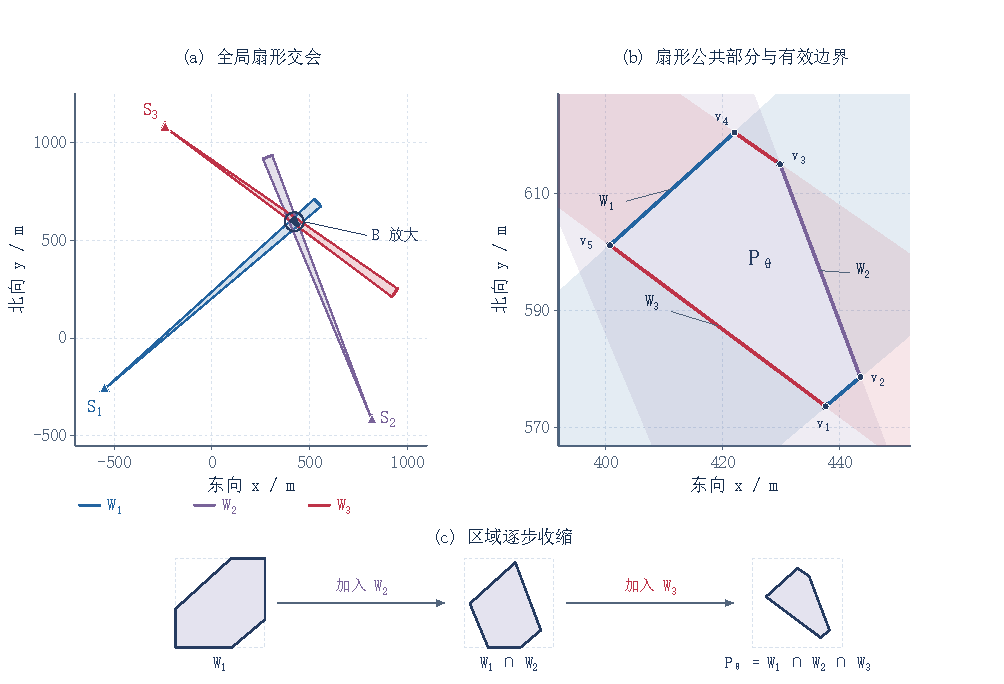
\includegraphics[width=1\linewidth]{fig1_sector_polygon.pdf}
    \caption{示向误差约束下定位多边形的构造过程}
    \label{fig:q1_modeling}
\end{figure}

\subsubsection{直径求解与半直径圆的充要判据}

首先判断 $Np\le b$ 的可行性。现有程序依次检验原点、原点到各边界直线的垂足及非平行边界交点，找到满足全部约束的候选点即判为非空。对非空交集，其有界性等价于衰退锥 $\{d:Nd\le0\}$ 只含零向量；程序逐一检验各边界的两个单位切向量，任一个满足 $Nd\le0$ 即判为无界。候选点检查的依据、函数对应及批量实验的不同实现见附录\ref{app:q1_implementation}。以下讨论非空有界情形。

设区域的极点为 $v_1,\ldots,v_h$。任意 $p,q\in P_\theta$ 均可写为顶点凸组合 $p=\sum_j\alpha_jv_j$、$q=\sum_k\beta_kv_k$，故
\[
\|p-q\|_2
\le\sum_{j,k}\alpha_j\beta_k\|v_j-v_k\|_2
\le\max_{j,k}\|v_j-v_k\|_2.
\]
右端可在区域内取到，因此
\begin{equation}
D=D(P_\theta)=\max_{p,q\in P_\theta}\|p-q\|_2
 =\max_{j,k}\|v_j-v_k\|_2.
\label{eq:q1_diameter}
\end{equation}
对逆时针排列的凸多边形顶点，可用经典旋转卡壳方法搜索对踵点对\cite{q1_toussaint1983}。对每条边 $(v_i,v_{i+1})$，推进对侧顶点至支撑三角形面积最大，并检查两端点到该顶点的距离；若相邻对侧顶点 $v_j,v_{j+1}$ 的支撑面积相等，则同时检查 $\{v_i,v_{i+1}\}\times\{v_j,v_{j+1}\}$ 的四组点对。这样将并列支撑纳入候选，可在线性时间内得到 $D$ 及一组直径端点 $A,B$。

当 $D>0$ 时，令 $M=(A+B)/2$。若存在半径为 $D/2$、圆心为 $c$ 的覆盖圆，则
\[
D=\|A-B\|_2\le\|A-c\|_2+\|B-c\|_2\le D.
\]
两处不等式均须取等号，于是 $c$ 位于线段 $AB$ 上且与两端等距，即 $c=M$。因此，允许自由选择圆心也不能改变半径 $D/2$ 下的判定；选取任意一组实际直径端点即可，无须为覆盖判定遍历全部直径对。

记 $B(c,r)$ 为闭圆盘。由圆盘的凸性，只需检验其是否包含全部顶点，得到
\begin{equation}
\begin{aligned}
P_\theta\subseteq B(M,D/2)
&\ \Longleftrightarrow\ \|v_j-M\|_2^2\le D^2/4\quad(\forall j)\\
&\ \Longleftrightarrow\ (v_j-A)\cdot(v_j-B)\le0\quad(\forall j).
\end{aligned}
\label{eq:q1_dot}
\end{equation}
其中第二个判据不需要逐点开方。为量化固定圆心下的覆盖缺口，定义
\begin{equation}
\kappa=\frac{\max_j\|v_j-M\|_2}{D/2}.
\label{eq:q1_kappa}
\end{equation}
由于直径端点到 $M$ 的距离均为 $D/2$，必有 $\kappa\ge1$；覆盖恰对应 $\kappa=1$。批量实验以 $\kappa\le1+10^{-9}$ 作为浮点计算中的覆盖判据；多条直径并列时的端点选取约定见附录\ref{app:q1_implementation}。

给定检测点坐标、示向度及误差界后，算法按“半平面构造—可行性与有界性判断—顶点提取—直径计算—覆盖判定”的顺序执行，输出区域状态、直径端点及覆盖结论。具体步骤如下。
\begin{enumerate}
\item 将观测角度归一化，按式\eqref{eq:q1_region}构造半平面；同向平行约束保留更严格者。检测不可行情况后返回“空集”；存在非零衰退方向时返回“无界”，不计算有限直径。
\item 对非空有界区域，按边界方向排序，用双端队列维护有效半平面。加入新约束时，反复删除使相邻交点落在新半平面外的队首、队尾边界，闭合后取相邻边界交点。去除重复点和共线冗余点，得到逆时针极点序列；平行及退化情形用边界交点枚举与约束回代复核。
\item 若只剩单点，返回 $D=0$ 及零半径覆盖圆，不定义 $\kappa$；若为线段，返回端点距离及端点中点圆。对正面积多边形，数值实现以全部顶点对枚举确定最终直径，并与卡壳结果交叉检查；差异超过 $10^{-7}\,\mathrm m$ 时报告异常。
\item 由一组直径端点计算 $M$，逐顶点检验式\eqref{eq:q1_dot}，输出直径、端点、圆心、覆盖结论及 $\kappa$。需要最优覆盖半径时，再求下文定义的最小覆盖圆。
\end{enumerate}

排序及双端队列半平面交的几何主流程为 $O(n\log n)$，上述含并列支撑处理的理论卡壳算法和逐顶点覆盖检查均为 $O(h)$。现有程序的可行点搜索、边界交点枚举并回代各为 $O(n^3)$，衰退方向检查为 $O(n^2)$，最终直径的全顶点对枚举为 $O(h^2)$；这些实现与核验成本均应计入运行代价。

\subsubsection{最小覆盖半径、理论界与可实现反例}

对任意候选圆心 $c$，定义覆盖整个定位区域所需的半径及其最小值：
\begin{equation}
R(c)=\max_j\|v_j-c\|_2,\qquad
R_{\min}=\min_{c\in\mathbb R^2}R(c),\qquad
C\in\mathop{\rm argmin}_{c\in\mathbb R^2}R(c).
\label{eq:q1_radius}
\end{equation}
$R(c)$ 是有限个欧氏距离函数的最大值，因而连续且凸，在最远顶点切换处可能不可微。最小覆盖圆优化的是圆心位置；固定直径中点后所需的半径则为 $R(M)=\kappa D/2$。任何覆盖圆都必须包含 $A,B$，故 $R_{\min}\ge D/2$，结合圆心唯一性可得
\begin{equation}
\text{半直径圆可覆盖}
\ \Longleftrightarrow\ R_{\min}=D/2
\ \Longleftrightarrow\ \kappa=1.
\label{eq:q1_equivalence}
\end{equation}

对 $D>0$ 的非空有界凸多边形，两类半径指标满足
\begin{equation}
1\le\kappa\le\sqrt3,\qquad
\frac12\le\frac{R_{\min}}{D}\le\frac1{\sqrt3}.
\label{eq:q1_bounds}
\end{equation}
固定中点的上界由平行四边形恒等式得到，最小覆盖半径的上界是平面 Jung 定理\cite{q1_jung1901}，可由最小覆盖圆的两点或三点支撑性质推得\cite{q1_welzl1991}。等边三角形以任一边为直径时，有 $\kappa=\sqrt3$、$R_{\min}=D/\sqrt3>D/2$，同时达到两个上界，说明一般凸多边形不存在半直径圆覆盖保证。中心对称集合则可由以其对称中心为圆心的半直径圆覆盖，可见覆盖性与具体形状有关。

最小覆盖圆（MEC）的主求解采用确定性增量支撑圆算法：按字典序处理顶点，遇到圆外点时，通过嵌套扫描更新单点圆、两点直径圆或三点外接圆，最坏复杂度为 $O(h^3)$。复核程序枚举全部两点直径圆和非共线三点外接圆，从包含所有顶点的候选圆中取半径最小者，直接实现为 $O(h^4)$。两者基于同一支撑性质，构成独立实现交叉核验。

为验证覆盖失败也会发生在本题楔形交会形成的区域中，构造表\ref{tab:q1_input}的三测点观测。该算例为合成输入，求解时仅使用测点坐标、示向度及误差界；完整精度数据保存在支撑材料中。
\begin{table}[H]
\centering
\caption{代表性合成算例的观测输入}
\label{tab:q1_input}
\begin{tabular}{crrr}
\toprule
检测点 & $x/\mathrm m$ & $y/\mathrm m$ & 示向度$/({}^\circ)$\\
\midrule
$S_1$ & $-550$ & $-260$ & $41.16915935$\\
$S_2$ & $820$ & $-420$ & $111.65365650$\\
$S_3$ & $-240$ & $1080$ & $324.23452557$\\
\bottomrule
\end{tabular}
\end{table}

该输入产生图\ref{fig:q1_modeling}中的凸五边形，直径端点为 $A=v_2$、$B=v_5$。表\ref{tab:q1_metrics}汇总关键结果。圆外顶点 $Q=v_1$ 满足
\[
(Q-A)\cdot(Q-B)=252.8066\,\mathrm m^2>0,
\]
使逐顶点覆盖不等式不成立，故直径圆不能覆盖该多边形。最小覆盖圆计算进一步得到 $R_{\min}>D/2$，与这一判定一致。



\begin{table}[H]
\centering
\caption{代表性五边形的几何计算结果}
\label{tab:q1_metrics}
\begin{tabular}{lrl}
\toprule
指标 & 数值 & 含义\\
\midrule
$M$ & $(429.8431,597.0774)\,\mathrm m$ & 直径中点坐标\\
$C$ & $(425.2719,595.5542)\,\mathrm m$ & 最小覆盖圆圆心坐标\\
$D$ & $49.2761\,\mathrm m$ & 区域直径\\
$D/2$ & $24.6380\,\mathrm m$ & 待检验的覆盖半径\\
$R(M)$ & $29.3230\,\mathrm m$ & 固定直径中点后的覆盖半径\\
$R_{\min}$ & $25.1048\,\mathrm m$ & 允许移动圆心的最小覆盖半径\\
$R(M)-D/2$ & $4.6850\,\mathrm m$ & 固定圆心的最大径向缺口\\
$R_{\min}-D/2$ & $0.4667\,\mathrm m$ & 优化圆心后的最小半径增量\\
$\kappa$ & $1.190152$ & 固定中点半径与半直径之比\\
$R_{\min}/D$ & $0.509472$ & 最小覆盖半径与直径之比\\
\bottomrule
\end{tabular}
\end{table}

图\ref{fig:q1_coverage}（A）比较定位五边形的直径圆与最小覆盖圆，径向短段标出圆外顶点 $Q$ 到直径圆的距离。两种半径增量具有不同的几何意义：$4.6850\,\mathrm m$ 是固定中点 $M$ 下的最大径向缺口，$0.4667\,\mathrm m$ 则是同时优化圆心后的最小补偿。

图\ref{fig:q1_coverage}（B）以相对最优圆心的位移 $\Delta x=c_x-C_x$、$\Delta y=c_y-C_y$ 为横纵轴，以曲面高度、颜色及等值投影表示覆盖半径 $R(c)$，单位均为米，参考高度为 $D/2$。曲面由 $R(c)$ 直接计算，用于展示圆心变化对覆盖半径的影响；最优圆心及半径由支撑圆算法确定并交叉核验。


\begin{figure}[H]
    \centering
    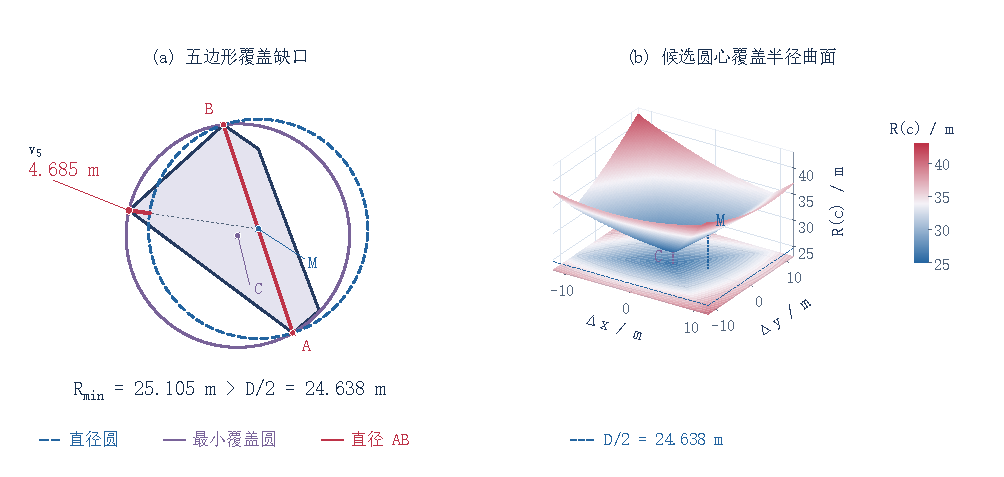
\includegraphics[width=0.95\linewidth]{fig2_coverage_surface.pdf}
    \caption{定位五边形的直径圆覆盖缺口与覆盖半径曲面}
    \label{app:q1_sampling}
\end{figure}

\subsubsection{数值核验与覆盖分布补充分析}

已有回归记录覆盖示向度跨零、近乎平行导致无界、矛盾观测空集、点与线段退化、误差边界及大坐标情形，并检查平移旋转不变性与加测后的直径单调性。另对分层抽取的 $600$ 组有界构型交叉检查区域顶点、原始角度约束、全顶点对直径及两份 MEC 实现的结果，所抽检样本在核验容差内一致；详细方法与记录见附录\ref{app:q1_sampling}。

在上述确定性分析基础上，合成实验进一步展示不同构型下覆盖比值的分布特征。对 $n=2,3,4,5$ 各生成 $60000$ 组观测，排除 $630$ 组无界构型后，以 $239370$ 组有界构型作分组统计；抽样机制与完整计数见附录\ref{app:q1_sampling}。

记 $\mathcal S_n$ 为检测点数为 $n$ 的有界样本集合，$N_n=|\mathcal S_n|$；将 $\kappa_s\le1+10^{-9}$ 的值归并为 $\widetilde\kappa_s=1$，其余保持原值，定义经验累积分布
\begin{equation}
\widehat F_n(t)=\frac{1}{N_n}\sum_{s\in\mathcal S_n}
\mathbf{1}\{\widetilde\kappa_s\le t\},\qquad 1\le t\le\sqrt3.
\label{eq:q1_ecdf}
\end{equation}
图\ref{fig:q1_kappa_ecdf}以无量纲阈值 $t$ 为横轴、$\widehat F_n(t)$ 为纵轴，各曲线按式\eqref{eq:q1_ecdf}保留经验分布的跳跃，$\sqrt3$ 为理论上界。$\widehat F_n(1)$ 是相应检测点数组中全部有界构型的可覆盖比例，$t>1$ 时的尾部 $1-\widehat F_n(t)$ 则表示固定直径中点的所需半径超过 $tD/2$ 的构型占比。

\begin{figure}[H]
    \centering
    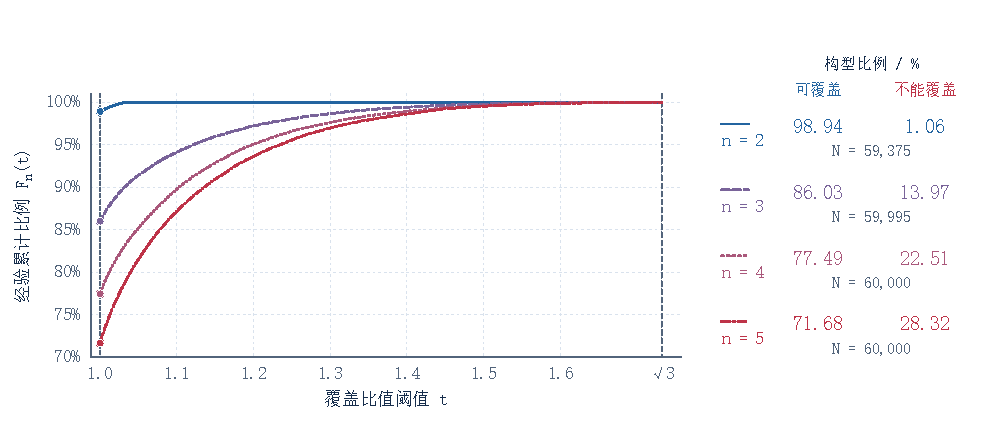
\includegraphics[width=0.9\linewidth]{fig3_kappa_ecdf.pdf}
    \caption{不同检测点数下覆盖比值 \(\kappa\) 的经验分布}
    \label{fig:q1_kappa_ecdf}
\end{figure}

图\ref{fig:q1_kappa_ecdf}在 $t=1$ 处的累计比例依次为 $98.94\%$、$86.03\%$、$77.49\%$ 和 $71.68\%$。当 $n=3,4,5$ 时，分别有 $2.77\%$、$4.92\%$、$6.36\%$ 的有界构型满足 $\kappa>1.2$，即固定直径中点时，覆盖半径须比半直径增加超过 $20\%$。各组频率以给定抽样机制为条件；对固定观测序列增加约束时，区域收缩，$D$ 与 $R_{\min}$ 均不增，不能将独立重抽样的组间差异解释为定位精度下降。

该判据可用于后续搜索策略：叠加目标区域及接收距离等物理约束后，应对实际候选区域重新计算 $D$ 与 $R_{\min}$。在最优圆心可达时，单次半径 $20\,\mathrm m$ 的探测能够覆盖该区域的充要条件为 $R_{\min}\le20\,\mathrm m$；$D\le40\,\mathrm m$ 只是必要条件。

\subsection{问题二：保守探测约束下的第二测点选择与候选区域构建}

问题一解决了如何根据两次示向结果确定定位区域及其直径。在此基础上，问题二需要进一步确定第二检测点的位置。第二检测点若离首测点过近，两次测向的交会角较小，定位精度提升有限；若移动过远，又可能超出部分潜在源点的有效探测范围。因此，本文先根据首测结果确定源点可能出现的区域，再综合目标圆域和接收距离限制，从可行位置中寻找最坏情况下定位区域直径尽可能小的第二检测点，最后通过方案比较和候选点复核确定实际布点位置。

\subsubsection{首测源集与保守探测约束}

沿用问题一的二维坐标、闭楔形 $W_i$ 和闭圆盘 $B(c,r)$ 记号。设首测点为 $S_1$，测得示向度为 $\theta_1$，未知源点为 $G$，待选第二测点为 $q=S_2$。示向误差界为 $\varepsilon=\pi/180$，有效接收半径为 $R\in[1000,1500]$ m，目标圆域为 $\mathcal D=B(O,1800)$。同一地点的示向误差在单个案例中固定；确定性模型仅使用误差界，不引入误差独立性假设。

成功取得首示向要求 $5<\|G-S_1\|_2\le1500$，故与观测一致的源集为
\[
K_1^{\rm obs}=\bigl[W_1\cap\mathcal D\cap B(S_1,1500)\bigr]\setminus B(S_1,5).
\]
为采用紧集上的距离极值计算，保守地加入距离恰为 $5$ m 的边界，定义计算源集
\begin{equation}
K_1=\bigl[W_1\cap\mathcal D\cap B(S_1,1500)\bigr]\setminus B^\circ(S_1,5),
\qquad K_1^{\rm obs}\subseteq K_1,
\label{eq:K1}
\end{equation}
其中 $B^\circ(c,r)$ 为开圆盘。边界的加入是计算上的保守外包，不表示距离等于 $5$ m 时能够获得示向。

标准化算例取 $S_1=O=(0,0)$、$\theta_1=0$。由于 $1500<1800$，目标圆域不截断首测角域，$K_1$ 为径向 $5\sim1500$ m、总张角 $2^\circ$ 的扇环。外弧两端间距为 $2\times1500\sin1^\circ\approx52.36$ m，而径向长度为 $1495$ m，说明首测主要压缩了横向不确定性，仍需通过第二次测向约束源距。

为保证任意可行源点在接收半径下限下仍能获得第二示向，采用保守布点域
\begin{equation}
\mathcal F=\left\{q:\
\sup_{G\in K_1}\|q-G\|_2\le1000,\quad
\inf_{G\in K_1}\|q-G\|_2>5,\quad
\max(|q_x|,|q_y|)\le2\times10^6\right\}.
\label{eq:feasible}
\end{equation}
首测成功还隐含 $R\ge\|G-S_1\|_2$，充分利用该信息时可将第一项放宽为逐源点满足 $\|q-G\|_2\le\max(1000,\|G-S_1\|_2)$。本文采用式\eqref{eq:feasible}给出的充分条件，使后续精度比较建立在第二次必可测向的前提上。

图\ref{fig:feasibility-explained}展示保守可行域，颜色表示探测裕度
\[
m(q)=1000-\sup_{G\in K_1}\|q-G\|_2.
\]
对标准扇环，可行测点的横坐标为正；源距平方对径向变量为凸函数，角向内部驻点若存在则为距离极小值，因此最远源距由扇环四个端点取得。图中仅绘出内弧下端点 $G_{\rm near}^{-}$ 和外弧上端点 $G_{\rm far}^{+}$ 的探测圆，着色区域则同时计入四端点约束及 $5$ m 近距排除条件。示例点 $q_{\rm out}=(1250,-500)$ m 距近端源点约 $1341.62$ m，故不可行。

\begin{figure}[H]
\centering
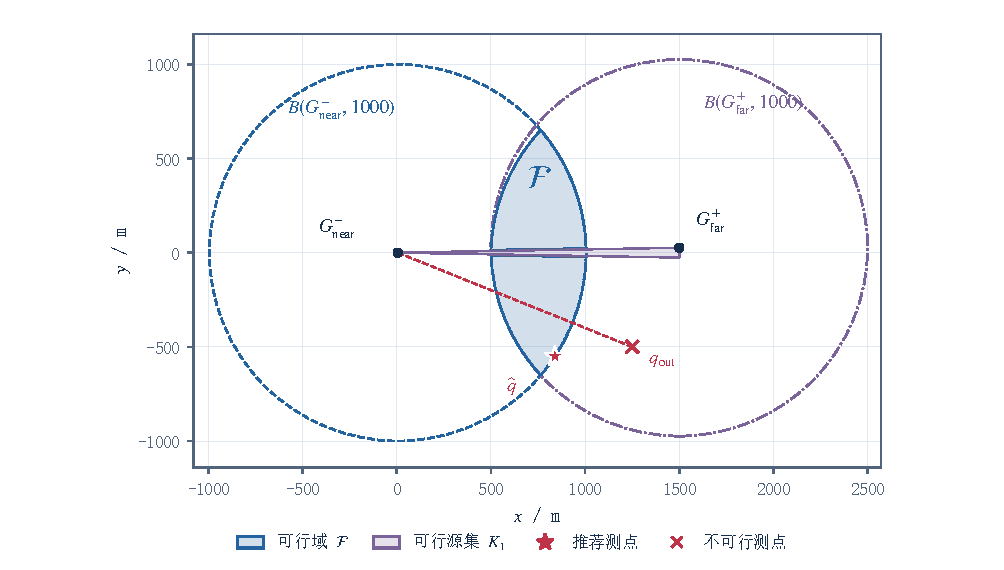
\includegraphics[width=\linewidth]{fig_feasibility_explained.pdf}
\caption{第二测点的保守探测可行域}
\label{fig:feasibility-explained}
\end{figure}

\subsubsection{布点目标与候选位置集合}

给定 $G\in K_1$ 和第二示向误差 $e\in[-\varepsilon,\varepsilon]$，第二示向为 $\theta_2=\arg(G-q)+e$。利用问题一的角域表示，构造用于直径评价的保守外包区域
\begin{equation}
\Omega(q;G,e)=W_1\cap W_2(q,\theta_2)\cap\mathcal D
\cap B(S_1,1500)\cap B(q,1500),
\label{eq:region}
\end{equation}
并以
\begin{equation}
D_2(q;G,e)=\max_{p,z\in\Omega(q;G,e)}\|p-z\|_2
\label{eq:diameter}
\end{equation}
衡量位置不确定性。式\eqref{eq:region}未挖去两次成功测向对应的近距禁区，因此完整观测信息下的源集包含于 $\Omega$，其直径不超过 $D_2$。保留凸外包区域可继续使用问题一的半平面交与直径算法，避免将含孔非凸集误作凸多边形处理。

图\ref{fig:intersection-explained}采用 $S_1=(0,0)$、$q=(830,-550)$、$G=(1100,0)$（单位均为 m）、$e=0$ 的独立构型。蓝色和紫色分别表示两次角域，红色为交会区域；右侧对同一区域作等比例放大，$A,B$ 为直径端点。该构型用于解释评价量，不是推荐测点的最坏情形。

\begin{figure}[H]
\centering
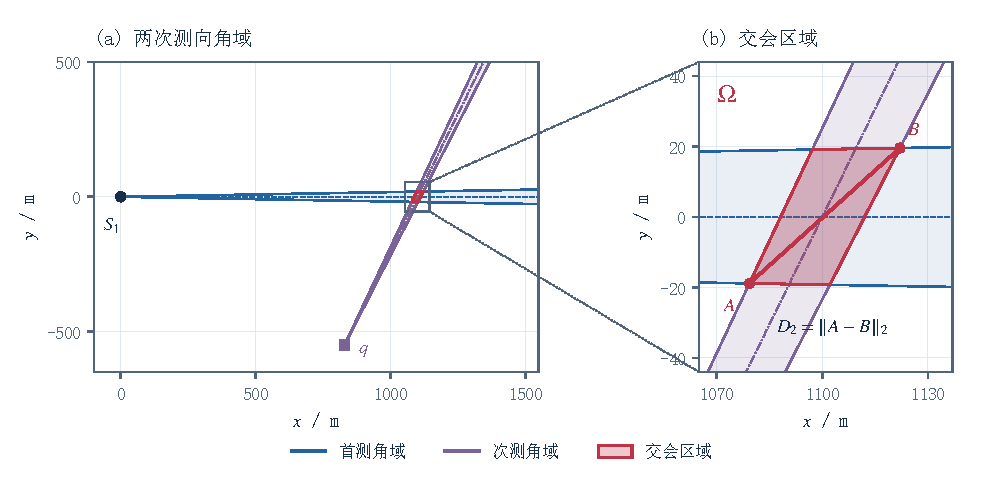
\includegraphics[width=\linewidth]{fig_intersection_explained.pdf}
\caption{两次测向的交会区域与定位直径}
\label{fig:intersection-explained}
\end{figure}

区域直径越小，仍可能包含源点的位置范围越小。沿用有界不确定传感器布设的极小极大思想\cite{tokekar2013}，分别定义标称目标与含示向误差的最坏目标：
\begin{align}
f_0(q)&=\sup_{G\in K_1}D_2(q;G,0),\label{eq:nominal}\\
f(q)&=\sup_{G\in K_1}\sup_{|e|\le\varepsilon}D_2(q;G,e).\label{eq:robust}
\end{align}
布点目标为
\begin{equation}
\min_{q\in\mathcal F} f(q).
\label{eq:minimax}
\end{equation}
即先评价每个测点的最不利构型，再选择最坏直径较小的位置。数值计算采用外接多边形近似圆盘，再进行半平面裁剪与旋转卡壳计算；几何外包保证固定构型下的保守性，但有限采样本身不构成连续最坏值或全局最优性的证明。

考虑计算量，初步搜索采用边界离散代理目标
\[
\widehat f_0(q)=\max_{G\in\mathcal B}D_2(q;G,0),
\]
其中 $\mathcal B$ 为 $K_1$ 两条径向边及内、外弧各取 $81$ 点形成的 $324$ 个采样条目。先用该目标筛选测点，再以统一的含误差最坏直径数值评价 $\widehat f(q)$ 比较推荐点与基准点。这样将计算较省的搜索与直接对应式\eqref{eq:robust}的比较分开，推荐依据不只来自代理目标。

对实际通行可采用的备选位置，取与推荐点对齐的 $5$ m 网格 $\mathcal G$，定义
\begin{equation}
\mathcal A_\delta=\{q\in\mathcal G\cap\mathcal F:
\widehat f_0(q)\le\widehat f_0(\widehat q)+\delta\},
\qquad \delta=5\ \mathrm m.
\label{eq:candidate}
\end{equation}
本文输出其中包含推荐点的一侧局部连通候选集合：从初始窗口中的合格点出发，逐点检验八邻域，直到不再出现相邻合格点。输出点均经过探测约束与标称性能核验；其凸包 $\mathcal H_\delta$ 仅辅助展示轮廓。阈值针对 $\widehat f_0$，不意味着鲁棒最坏直径只增加 $5$ m，也不将网格点之间的位置自动判为合格。

\subsubsection{数值求解与对比验证}

先在 $x\in[450,1050]$ m、$y\in[-800,800]$ m 内以 $10$ m 步长进行可行网格搜索，再从最优网格点出发进行局部模式搜索。步长逐级减半至 $0.0069$ m，得到
\[
\widehat q=(839.70703125,-550.60546875)\ \mathrm m,
\qquad \widehat f_0(\widehat q)=108.329\ \mathrm m.
\]
搜索终止尺度不表示定位误差或最优点误差。推荐点的移动距离为 $1004.13$ m，与首示向夹角为 $-33.25^\circ$；以 $5$ m/s 行走时需 $200.83$ s。其最近源距为 $535.88$ m，探测裕度仅为 $0.000208$ m，几乎处于约束边界。计算使用完整精度坐标，表中舍入值仅用于展示；实际存在落点偏差时，应选取裕度更大的候选位置并重新核验。

为使所有方案按相同指标比较，注意式\eqref{eq:region}中 $G,e$ 仅通过第二示向 $\theta_2$ 进入几何计算。对本次比较的下侧可行测点，$K_1$ 连通且不包含测点，其无跨角度分支的方位像为闭区间 $I(q)$。区间端点由扇环端点与可能的圆弧切点求得，叠加误差后所有可能示向构成
\[
\Theta(q)=I(q)+[-\varepsilon,\varepsilon].
\]
因此可直接扫描 $\Theta(q)$ 评价原有鲁棒目标，避免仅在源集边界上寻找最坏源点。对各方案统一采用 $1001$ 点和 $2001$ 点两级示向扫描，并在每级最高的六个局部峰附近加密；对推荐点另用 $4001$ 点复核。两级峰值加密结果的差异均小于 $2\times10^{-6}$ m，推荐点的再次复核变化小于 $2\times10^{-7}$ m。这些差异衡量本次数值扫描的稳定性，不作为解析误差界。

\begin{table}[htbp]
\centering\small
\caption{第二测点方案的同口径比较}
\label{tab:result}
\begin{tabular}{lrrrrr}
\toprule
方案 & $q_x$/m & $q_y$/m & $\widehat f$/m & 移动距离/m & 探测裕度/m\\
\midrule
推荐点 & $839.707$ & $-550.605$ & $110.974$ & $1004.13$ & $0.0002$ \\
邻近点A & $829.707$ & $-550.605$ & $112.327$ & $995.78$ & $8.332$ \\
邻近点B & $839.707$ & $-540.605$ & $111.864$ & $998.68$ & $5.472$ \\
邻近点C & $829.707$ & $-560.605$ & $111.453$ & $1001.35$ & $2.744$ \\
邻近点D & $849.707$ & $-530.605$ & $111.406$ & $1001.77$ & $2.420$ \\
横向中点基准 & $752.500$ & $-500.000$ & $129.343$ & $903.47$ & $86.064$ \\
长基线基准 & $800.000$ & $-600.000$ & $112.133$ & $1000.00$ & $3.942$ \\
短基线基准 & $750.000$ & $-50.000$ & $512.669$ & $751.66$ & $246.368$ \\
\bottomrule
\end{tabular}
\end{table}

表\ref{tab:result}中的四个邻近点用于检查局部位置扰动，横向中点、长基线和短基线三种简单布点作为参照。八个方案均满足式\eqref{eq:feasible}，推荐点的最坏直径数值评价最小，为 $110.974$ m；长基线基准为 $112.133$ m，短基线基准为 $512.669$ m。这说明当前测点兼顾了对整个源集的探测与交会几何，而较短的移动距离可能保留明显更大的不确定性。该比较支持保留当前推荐点，但不宣称它是整个可行域上的全局最优解。

同一坐标下，代理值 $108.329$ m 与复核值 $110.974$ m 相差约 $2.4\%$。本次扫描找到的峰值位于无误差可达区间 $I(q)$ 内；例如取内部源点 $G\approx(1448.050,0)$ m、$e=0$，代入原几何核即可得到 $D_2\approx110.974$ m。这说明不能把这部分差距直接解释为第二示向误差的影响，首测源集的边界离散确实遗漏了更不利的源距构型。方案比较、统计样本和候选数据均使用上述完整精度测点坐标。

初始候选窗口为推荐点横向 $\pm80$ m、纵向 $\pm160$ m，含 $235$ 个合格网格点。边界核验发现左侧仍有合格延续，例如窗口外的 $(754.707,-640.605)$ m 对应 $\widehat f_0=112.817$ m。经八邻域扩展后，共得到 237 个合格点，比初始窗口增加 2 个；所有合格点的八邻域均已检查，因而不再把原窗口边缘作为该网格连通分支的性能边界。此结论针对当前 $5$ m 网格连通分支，不排除其他不相连的合格区域，也不认证连续近优区域。

图\ref{fig:k1}同时展示真实合格网格点、标称性能等值线和辅助凸包。背景颜色来自已计算的 $\widehat f_0(q)$；节点间插值只用于显示。两条等值线分别对应 $\widehat f_0(\widehat q)+2.5$ m 和 $\widehat f_0(\widehat q)+5$ m，后者阈值为 $113.329$ m。扩展后的凸包有 16 个顶点、面积约 5525.0 m$^2$。应从已核验的离散点中结合通行条件与探测裕度选取实际位置，连续调整后的落点需重新计算，不能仅凭处于凸包内部判断可用。

\begin{figure}[htbp]
\centering
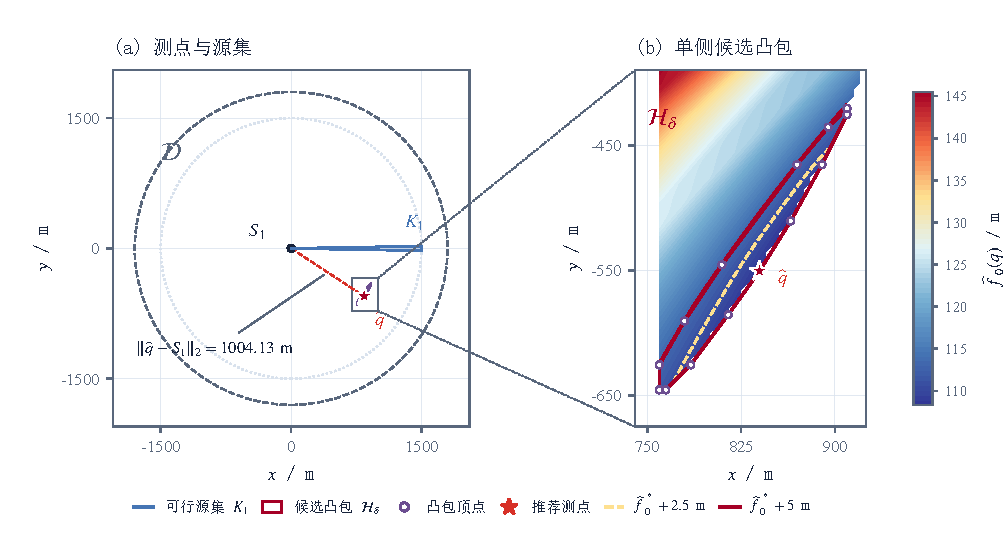
\includegraphics[width=\linewidth]{fig_k1_combined.pdf}
\caption{首测可行源集与第二测点候选区域}
\label{fig:k1}
\end{figure}

对一般首测点与首示向，令
\begin{equation}
p'=Q^{\mathsf T}(p-S_1),\qquad
Q=\begin{pmatrix}\cos\theta_1&-\sin\theta_1\\
\sin\theta_1&\cos\theta_1\end{pmatrix},
\label{eq:transform}
\end{equation}
则目标圆心变为 $O'=Q^{\mathsf T}(O-S_1)$。当目标圆域不截断首测扇环时，可复用标准化算例的源集与测点，再以 $S_2=S_1+Q\widehat q$ 还原并核对全局坐标限制；$\|S_1-O\|_2\le300$ m 是保证整个 $1500$ m 接收圆盘包含于目标圆域的一个充分条件，并非必须首测点位于圆心。若目标圆域截断首测扇环，则须更新 $K_1$ 并重新求解。未截断时上下侧关于首示向轴对称，故推荐点的镜像同样可用。

本问没有额外移动时间预算。对完整扇环，由最远接收端与最近源距端的三角不等式可得 $500\le\|q-S_1\|_2\le1005$ m，对应 $100\sim201$ s。这只是必要范围，不保证端点可达；推荐点接近其上界，说明当前精度目标偏好较长的可行基线。

\subsubsection{补充概率假设下的定位效果评估}

上述模型控制最不利构型。为补充典型表现，假设首测成功后的源点在 $K_1$ 上按面积均匀分布，第二示向误差独立服从 $U(-1^\circ,1^\circ)$。使用随机种子 $20260913$，取 $r=\sqrt{U(5^2,1500^2)}$、方位角 $U(-1^\circ,1^\circ)$ 生成 $1000$ 个合成源点，并逐样本计算保守外包区域的直径与形心。这里的独立均匀误差是补充实验假设，不改变确定性模型中的误差界；每个源点及第二示向均仅抽样一次。

由于 $\widehat q\in\mathcal F$、$R\ge1000$ m，所有可行源点均满足第二次接收与非近距条件，故本实验的条件探测概率为 $1$。接收半径分布和失败损失不影响该测点评价，不再引入这些概率机制。取损失 $L=D_2$，以条件风险价值
\begin{equation}
\operatorname{CVaR}_{\alpha}(L)=\min_{\eta}\left\{\eta+
\frac{\mathbb E[(L-\eta)_+]}{1-\alpha}\right\}
\end{equation}
描述尾部不确定性；$\alpha=0.95$ 时，样本估计取最大 $50$ 个直径的均值。

本次样本的平均直径为 61.37 m，中位数为 54.19 m，$95\%$ 分位数为 105.94 m，$\operatorname{CVaR}_{0.95}$ 为 108.53 m，样本最大值为 110.93 m。典型直径低于最坏扫描值，但远距离源点仍保留较大的位置不确定性，分段结果见表\ref{tab:bands}。

\begin{table}[htbp]
\centering\small
\caption{合成样本在不同源距区间的定位效果}
\label{tab:bands}
\begin{tabular}{lrrrr}
\toprule
源距区间/m & 样本数 & 平均直径/m & $p_{95}$/m & 形心20 m命中率/\%\\
\midrule
$(5,300)$ & $39$ & $53.94$ & $60.25$ & $82.1$ \\
$[300,600)$ & $126$ & $42.73$ & $48.20$ & $99.2$ \\
$[600,900)$ & $189$ & $36.32$ & $38.34$ & $100.0$ \\
$[900,1200)$ & $293$ & $53.09$ & $67.33$ & $88.7$ \\
$[1200,1500]$ & $353$ & $89.12$ & $108.90$ & $58.4$ \\
\bottomrule
\end{tabular}
\end{table}

记 $c_\ell$ 为第 $\ell$ 个保守外包区域的面积形心，形心落点的 $20$ m 命中率（合成样本）定义为
\[
\widehat p_{20}=\frac{1}{1000}\sum_{\ell=1}^{1000}
\mathbf1\{\|c_\ell-G_\ell\|_2\le20\}.
\]
本次总体命中率为 81.2\%。该量依赖合成真值，只回答形心落点在多少样本中接近源点，不提供整个定位区域均可清除的保证。按照问题一的覆盖性判据，若需对全部可能源点给出半径 $20$ m 的几何保证，应另行核验最小覆盖圆半径是否不超过 $20$ m；该指标与形心命中率不能混用，也不能以 $D_2/2$ 直接替代最小覆盖半径。


\subsection{问题三模型的建立与求解}


\subsection{问题四模型的建立与求解}
\subsubsection{模型假设、数学归类与总体思路}

\noindent\textbf{1. 模型假设}

在题设条件基础上作如下本问专属假设：各干扰源在被清除前位置、频道、有效接收半径、源类型及发射方向保持不变，且不同干扰源占用不同频道；目标圆域内不存在未给出的通行障碍，机器狗位置控制准确，并以 $5\,\mathrm{m/s}$ 的速度沿两点间直线路径移动，移动过程中不进行检测；测向误差仅满足题设给出的 $\pm1^\circ$ 有界条件，不额外假定其概率分布；概率层所需的位置、半径、源类型和朝向先验取自模拟器公开生成规则，仅用于探点选择、路径排序和停止风险评价，不参与已发现频道的确定性清除判据。

\noindent\textbf{2. 模型的数学归类}

本问可归类为\textbf{部分可观测混合状态下的序贯决策与滚动路径优化问题}。

\begin{table}[H]
\centering
\caption{问题四模型主要符号}
\label{tab:q4_symbols}
\begin{tabular}{cl}
\toprule
符号 & 含义 \\
\midrule
$\mathcal C$ & 频道集合 $\{1,2,\ldots,20\}$ \\
$\mathcal C_t^{+}$ & 已发现的频道集合 \\
$\mathcal C_t^{\rm clr}$ & 已清除的频道集合 \\
$\mathcal C_t^{?}$ & 尚未确认的频道集合 \\
$\xi_c=(z_c,G_c,R_c,d_c,\phi_c)$ & 频道 $c$ 的联合状态变量 \\
$z_c$ & 表示频道 $c$ 是否存在干扰源 \\
$G_c=(x_c,y_c)$ & 干扰源位置坐标 \\
$R_c$ & 有效接收半径，$R_c\in[1000,1500]$ m \\
$d_c$ & 源类型：$d_c=0$ 为全向源，$d_c=1$ 为定向源 \\
$\phi_c$ & 定向源发射方向 \\
$u(\phi_c)$ & 定向源方向向量 $(\cos\phi_c,\sin\phi_c)^{\mathsf T}$ \\
$V_c(q;\xi_c)$ & 检测点 $q$ 处的可见性判定函数 \\
$q$ & 当前检测点位置 \\
$T$ & 虚拟总时间 \\
$N_{\rm clr}$ & 已清除频道数，$N_{\rm clr}=|\mathcal C_T^{\rm clr}|$ \\
$\bar T$ & 平均定位清除时间，$\bar T=T/N_{\rm clr}$ \\
$\mathcal P_c,\mathcal N_c,\mathcal F_c$ & 正观测点、无信号点与清除失败点集合 \\
$\mathcal H_t$ & 截至时刻 $t$ 的历史观测集合 \\
$\mathcal B_c^{\rm out}$ & 仅依赖正示向构造的保守位置外包 \\
$r_{\rm clr}=20$ m & 清除失败后可严格排除的清除半径 \\
$s_c$ & 频道 $c$ 的生存似然 \\
$P_{\rm rem}$ & 仍有未发现活动源的后验风险 \\
\bottomrule
\end{tabular}
\end{table}

问题四的核心困难在于：多频道源数未知、定向源使无信号观测具有歧义，同时机器人移动成本较高。为此，本文采用“确定性外包保证清除安全 + 粒子后验提高搜索效率 + 动态路径规划降低移动时间”的双层在线策略。

\subsubsection{建模思路与优化目标}

记频道集合为 $\mathcal C=\{1,2,\ldots,20\}$，已经发现、已经清除和尚未确认的频道集合分别记为 $\mathcal C_t^{+}$、$\mathcal C_t^{\rm clr}$ 和 $\mathcal C_t^{?}$。对频道 $c$ 定义未知状态
\begin{equation}
\xi_c=(z_c,G_c,R_c,d_c,\phi_c),
\label{eq:q4_state}
\end{equation}
其中，$z_c\in\{0,1\}$ 表示频道是否存在干扰源，$G_c=(x_c,y_c)$ 为源点位置，$R_c\in[1000,1500]$ m 为有效接收半径，$d_c=0$ 和 $d_c=1$ 分别表示全向源和定向源，$\phi_c$ 为定向源发射方向。令
\[
u(\phi_c)=(\cos\phi_c,\sin\phi_c)^{\mathsf T}.
\]
机器狗位于 $q$ 时，频道 $c$ 的信号可见条件为
\begin{equation}
V_c(q;\xi_c)=z_c\,
\mathbf 1\!\left\{\|q-G_c\|_2\le R_c\right\}
\left[(1-d_c)+d_c\mathbf 1\!\left\{(q-G_c)^{\mathsf T}u(\phi_c)\ge0\right\}\right].
\label{eq:q4_visibility}
\end{equation}
式\eqref{eq:q4_visibility}中的内积约束描述定向源前方 $180^\circ$ 的有效辐射区域。若 $V_c=0$，检测结果为无信号；若 $V_c=1$ 且机器狗未进入近距区域，则获得误差不超过 $\varepsilon=1^\circ$ 的示向度；进入近距区域后返回近距信息，可直接尝试清除。

检测点既可能在有效接收圆外，也可能虽处于接收半径内却落在定向源的背向半平面。两种情形返回相同的无信号观测，因而单个无信号点只给出析取信息，不能像全向源情形那样直接排除其邻域。

设机器狗依次访问 $q_0,q_1,\ldots,q_M$，移动速度为 $v=5$ m/s。记第 $j$ 次动作产生的频道切换、测量和清除用时分别为 $t_j^{\rm sw}$、$t_j^{\rm mea}$ 和 $t_j^{\rm clr}$，则任务虚拟总时间为
\begin{equation}
T=\sum_{j=0}^{M-1}\frac{\|q_{j+1}-q_j\|_2}{v}
+\sum_j\left(t_j^{\rm sw}+t_j^{\rm mea}+t_j^{\rm clr}\right).
\label{eq:q4_time}
\end{equation}
本文采用分层优化目标。第一层目标为尽可能发现并清除全部真实干扰源；在满足完整性要求的策略中，第二层目标最小化平均定位清除时间
\begin{equation}
\bar T=\frac{T}{N_{\rm clr}},
\qquad N_{\rm clr}=|\mathcal C_T^{\rm clr}|.
\label{eq:q4_average_time}
\end{equation}
因此，算法不以牺牲漏源风险换取较小的 $\bar T$，而仅在搜索完整性得到控制后优化移动、检测和清除时间。由于真实源数在任务结束前未知，本文不预先固定待清除源数，而采用后验漏源风险和题设最大源数共同控制停止。


\subsubsection{双层信念表示：确定性外包与概率后验}

沿用问题一的闭楔形记号。频道 $c$ 在检测点 $q_i$ 获得示向度 $\theta_{ic}$ 后，源点必须满足正示向约束
\begin{equation}
G_c\in W(q_i,\theta_{ic})\cap B(q_i,R_c),
\qquad
|\operatorname{wrap}(\arg(G_c-q_i)-\theta_{ic})|\le\varepsilon,
\label{eq:q4_positive_bearing}
\end{equation}
若该源为定向源，还须满足正面半平面约束 $(q_i-G_c)^{\mathsf T}u(\phi_c)\ge0$。记正观测点、无信号点和清除失败点集合分别为 $\mathcal P_c$、$\mathcal N_c$ 和 $\mathcal F_c$。一旦频道获得过正观测，便有 $z_c=1$；此时无信号点 $q_i\in\mathcal N_c$ 对应析取约束
\begin{equation}
\|q_i-G_c\|_2>R_c
\quad\lor\quad
\left[d_c=1\ \land\ (q_i-G_c)^{\mathsf T}u(\phi_c)<0\right],
\label{eq:q4_no_signal}
\end{equation}
即在有效半径之外或位于定向源的背向半平面。清除失败则可严格排除
\begin{equation}
G_c\notin B(q_i,r_{\rm clr}),\qquad q_i\in\mathcal F_c.
\label{eq:q4_clear_failure}
\end{equation}

为保证清除环节不因近似后验而漏掉真实位置，构造只依赖正示向的保守位置外包
\begin{equation}
\mathcal B_c^{\rm out}
=\mathcal D\cap
\bigcap_{(q_i,\theta_{ic})\in\mathcal P_c}
\left[W(q_i,\theta_{ic})\cap B(q_i,1500)\right].
\label{eq:q4_outer_belief}
\end{equation}
真实源点必位于 $\mathcal B_c^{\rm out}$ 内。因而本文不利用无信号观测直接裁剪 $\mathcal B_c^{\rm out}$，只使用正示向和严格清除失败信息进行确定性排除；数值实现以外接正多边形逼近圆域并进行半平面裁剪，避免内接离散误删真实源点。

确定性外包不含无信号信息，无法评价“去哪里最可能发现新源”。为此，概率层采用序贯蒙特卡洛（粒子滤波）近似\cite{arulampalam2002,thrun2005}：按模拟器公开生成规则抽取 $L$ 个状态粒子 $\xi_c^{(\ell)}$，并以与历史观测的相容性赋权
\begin{equation}
w_{c\ell}^{(t)}\propto w_{c\ell}^{(0)}
\prod_{h\in\mathcal H_t}
\mathbf 1\!\left\{\xi_c^{(\ell)}\text{ 与观测 }h\text{ 相容}\right\},
\label{eq:q4_particle_weight}
\end{equation}
据此估计候选检测点 $q$ 处仍能发现频道 $c$ 的后验可见率
\begin{equation}
p_c(q)=P\bigl(\text{在 }q\text{ 可检测到频道 }c\mid\mathcal H_t\bigr)
\approx\frac{\sum_{\ell=1}^{L}w_{c\ell}^{(t)}V_c(q;\xi_c^{(\ell)})}{\sum_{\ell=1}^{L}w_{c\ell}^{(t)}}.
\label{eq:q4_probe_probability}
\end{equation}
将 $q$ 插入路径相邻节点 $a,b$ 之间所增加的路程为 $\Delta L(q\mid a,b)=\|a-q\|_2+\|q-b\|_2-\|a-b\|_2$。预规划阶段以“单位时间发现收益”排序
\begin{equation}
J_1(q)=\frac{p_c(q)}{t_0+\Delta L(q)/v},
\label{eq:q4_probe_score1}
\end{equation}
尾部补查阶段以“发现概率减去移动代价”排序
\begin{equation}
J_2(q)=p_c(q)-\lambda\frac{\|q-q_t\|_2}{v}.
\label{eq:q4_probe_score2}
\end{equation}
逐次选取最高价值点后，对已被该点覆盖的粒子降权，使后续探点优先覆盖尚未涉及的后验模态。需要强调，粒子后验仅承担效率优化，不参与确定性清除保证：即使粒子近似失效或排序有误，最终清除仍回到 $\mathcal B_c^{\rm out}$ 与保守走廊，正确性不受影响。这也正是本文将确定性信息与概率信息分离的原因——确定性可行域仅由不会错误排除真实源的观测构造，用于决定清除覆盖；粒子后验仅用于探点选择和访问顺序优化。

\subsubsection{单频道自适应定位与清除}

当频道 $c$ 获得不少于两条正示向信息时，记第 $i$ 条示向的单位方向向量及其法向量分别为
\[
e_i=(\cos\theta_{ic},\sin\theta_{ic})^{\mathsf T},\qquad
n_i=(-\sin\theta_{ic},\cos\theta_{ic})^{\mathsf T}.
\]
忽略角度误差时，每条示向对应一条经过检测点 $q_i$、方向为 $e_i$ 的直线。为获得用于路径排序和快速尝试的点估计，采用多站被动定位中的最小二乘交会方法\cite{torrieri1984}，最小化候选源点到各示向中心线的垂直距离平方和：
\begin{equation}
\widehat G_c
=\arg\min_{G\in\mathcal D}
\sum_{i\in\mathcal P_c}
\left[n_i^{\mathsf T}(G-q_i)\right]^2.
\label{eq:q4_ls}
\end{equation}

需要强调的是，$\widehat G_c$ 仅为用于提高搜索效率的点估计，并不承担真实源位置的确定性覆盖保证。示向误差所对应的位置不确定性仍由保守外包 $\mathcal B_c^{\rm out}$ 描述。

为衡量多站交会的几何稳定性，定义已有示向之间的最大有效锐交会角
\begin{equation}
\alpha_c=
\max_{i\ne j}
\angle_{\rm acute}(e_i,e_j).
\label{eq:q4_acute_angle}
\end{equation}
当 $\alpha_c$ 较大时，不同示向对源位置具有较强的交叉约束；当示向近乎平行时，即使最小二乘问题仍有数值解，其位置误差也可能被显著放大，因此不直接依据 $\widehat G_c$ 作清除判定。

对保守外包 $\mathcal B_c^{\rm out}$ 计算最小覆盖圆 $(o_c,\rho_c)$。若满足
\begin{equation}
\rho_c\le r_{\rm clr},
\label{eq:q4_mec_clear}
\end{equation}
则有
\[
\mathcal B_c^{\rm out}\subseteq B(o_c,r_{\rm clr}),
\]
因此机器狗移动至 $o_c$ 即可一次覆盖全部可能的真实源位置。该分支提供严格的确定性清除保证，与问题一中的最小覆盖圆结论一致。

若式\eqref{eq:q4_mec_clear}尚不满足，但交会几何较好，即
\[
\alpha_c\ge\alpha_{\min},
\qquad
\rho_c\le\rho_{\rm fast},
\]
则首先利用 $\widehat G_c$ 进行低成本快速尝试，并可在其邻域设置少量局部清除点。该步骤仅用于降低平均定位时间，不视为完整覆盖：若快速清除失败，仅依据清除失败位置按式\eqref{eq:q4_clear_failure}排除其 $r_{\rm clr}$ 邻域，并保留其余保守可行区域。

当仅获得一条示向、示向线近乎平行，或上述快速尝试未成功时，算法转入保守覆盖分支。设最新正观测点为 $q_0$，中心示向单位向量为 $e$，对应法向量为 $n$。根据当前保守外包 $\mathcal B_c^{\rm out}$ 构造清除点集合 $\mathcal Q_c^{\rm cor}$，并持续增加覆盖点直至满足
\begin{equation}
\sup_{G\in\mathcal B_c^{\rm out}}
\min_{q\in\mathcal Q_c^{\rm cor}}
\|G-q\|_2
\le r_{\rm clr}.
\label{eq:q4_corridor_cover}
\end{equation}
因此，对任意仍可能的真实源位置 $G\in\mathcal B_c^{\rm out}$，至少存在一个清除点与其距离不超过 $r_{\rm clr}$。式\eqref{eq:q4_corridor_cover}构成单频道清除完整性的最终保证。

实际执行过程中，机器狗按照由近及远的顺序访问 $\mathcal Q_c^{\rm cor}$。每次清除失败后，利用式\eqref{eq:q4_clear_failure}严格排除当前位置附近区域，并在当前位置重新测向；若得到新的正示向，则立即更新 $\mathcal B_c^{\rm out}$、重新计算式\eqref{eq:q4_ls}以及最小覆盖圆。由此，随着新观测不断加入，原计划的远端覆盖点可以被重新评估，从而避免机械遍历整个初始角域。

综上，单频道策略按照
\[
\text{最小覆盖圆保证清除}
\;\longrightarrow\;
\text{稳定交会下快速尝试}
\;\longrightarrow\;
\text{保守区域完整覆盖}
\]
的三级结构自适应切换。前两级用于降低平均移动与清除时间，最后一级负责保证在不利几何构型下仍不遗漏保守外包中的可能源点，其决策过程如图\ref{fig:q4-channel-decision}所示。

\begin{figure}[H]
\centering
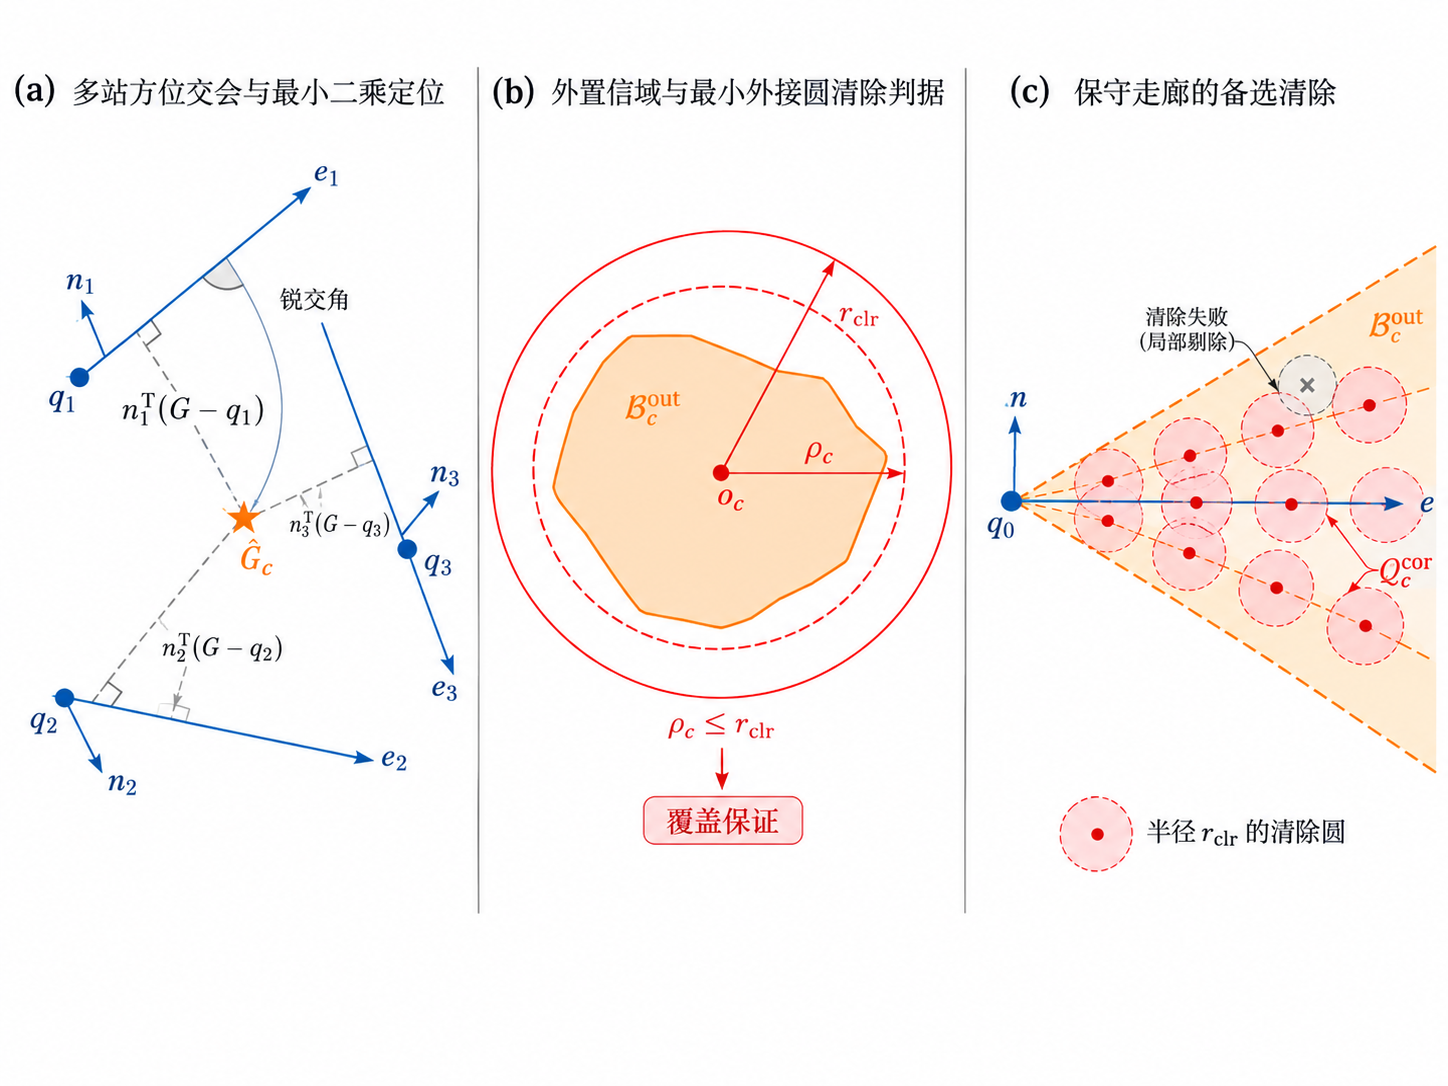
\includegraphics[width=\linewidth]{figures/q4_single_channel_adaptive.png}
\caption{单频道自适应定位与清除过程示意}
\label{fig:q4-single-channel-adaptive}
\end{figure}



\subsubsection{动态任务集与滚动路径优化}

对每个已发现但尚未清除的频道，依据式\eqref{eq:q4_ls}或最小覆盖圆圆心得到路线目标 $g_c$；将这些清除目标与后验补查点共同构成动态任务点集
\begin{equation}
\mathcal V_t=\{g_c:c\in\mathcal C_t^{+}\setminus\mathcal C_t^{\rm clr}\}
\cup\mathcal Q_t^{\rm probe}.
\label{eq:q4_task_set}
\end{equation}
清除目标随观测动态增长，访问顺序是任务点实时更新的动态旅行商问题。本文从当前位置出发，以构造型最近邻启发式生成开放路径，再以 2-opt 局部交换消除交叉与回头路\cite{croes1958,rosenkrantz1977}，近似求解
\begin{equation}
\min_{\pi}\sum_{j=0}^{|\mathcal V_t|-1}
\|q_{\pi_{j+1}}-q_{\pi_j}\|_2.
\label{eq:q4_route}
\end{equation}

为降低独立普查产生的额外移动代价，本文进一步将清除终点复用为未知频道扫描点。每成功清除一个干扰源后，机器狗不立即离开，而在当前清除位置扫描仍未知的频道；若发现新源，则把新目标加入式\eqref{eq:q4_task_set}并重新规划剩余路线，形成“清除已有源 $\longrightarrow$ 清除点扫描未知频道 $\longrightarrow$ 发现新源 $\longrightarrow$ 重新定位与规划”的滚动过程。清除点通常分散在目标圆域内，将其兼作检测点能够取得较大的观测基线，而无需为普查单独承担全部移动成本，这是降低总时间的主要机制。

程序首先在原点扫描全部频道；若中心点发现数不足以表明高密度场景，则继续访问若干分散普查点（半径 $r_{\rm scout}$，见表\ref{tab:q4_params}）。上述阈值及补查预算均为离线调参得到的算法参数，其稳健性将在模型检验部分通过阈值扰动与策略消融加以验证。

\subsubsection{未发现源风险与停止准则}

对未知频道 $c$，定义其生存似然为：在“频道确有活动源”的假设下，该源在全部历史无信号观测中始终未被发现的概率
\begin{equation}
s_c=P(\mathcal H_t^c\mid z_c=1)
\approx\frac{1}{L}\sum_{\ell=1}^{L}
\mathbf 1\!\left\{\xi_c^{(\ell)}\text{ 与全部历史观测相容}\right\},
\label{eq:q4_survival}
\end{equation}
其中 $\mathcal H_t^c$ 为频道 $c$ 的历史无信号观测，求和仅覆盖 $z_c^{(\ell)}=1$ 的粒子。设当前已发现 $k$ 个频道、未知频道数为 $U$。依据源总数位于 $10$--$16$ 且活动频道等可能的生成先验，将各未知频道的生存似然 $s_1,\ldots,s_U$ 按基本对称多项式
\begin{equation}
e_m(s_1,\ldots,s_U)=\sum_{1\le i_1<\cdots<i_m\le U}\prod_{j=1}^{m}s_{i_j},\qquad e_0=1
\label{eq:q4_symmetric}
\end{equation}
组合，可得未知频道中恰有 $m$ 个活动源的未归一化后验权重
\begin{equation}
\omega_m=\frac{e_m(s_1,\ldots,s_U)}{\binom{20}{k+m}},
\quad m\in\left[\max(0,10-k),\min(16-k,U)\right],
\label{eq:q4_count_weight}
\end{equation}
于是仍有未发现活动源的后验风险为
\begin{equation}
P_{\rm rem}=P(N_{\rm unseen}\ge1\mid\mathcal H_t)=1-\frac{\omega_0}{\sum_m\omega_m},
\label{eq:q4_remaining_risk}
\end{equation}
当 $m=0$ 不在允许范围时取 $P_{\rm rem}=1$。$P_{\rm rem}$ 用于决定是否值得进行远距离尾部补查，但不作为“未知频道均为空”的确定性证明。

综合而言，在线策略在以下任一条件满足时停止新增搜索：一是已发现题设最大数量 $16$ 个源；二是剩余真实运行时间低于安全裕量；三是 $P_{\rm rem}$ 已低于设定阈值且不存在强制补查分支。停止搜索前，对所有已发现但尚未清除的频道继续执行交会定位或保守走廊清除。

\subsubsection{在线算法流程}

问题四的滚动求解过程如下：

\noindent 1) 初始化各频道的空、全向、定向三类状态分支，在原点完成全频道扫描；

\noindent 2) 根据中心点发现数量选择分散普查或动态联合路径；

\noindent 3) 每获得示向、近距、无信号或清除失败反馈后，分别更新保守外包与联合粒子后验；

\noindent 4) 对已发现频道优先进行多站交会，满足式\eqref{eq:q4_mec_clear}时直接清除，否则执行局部探点或保守走廊；

\noindent 5) 在清除终点扫描未知频道，并把新发现源及高价值后验探点加入任务点集，重新执行最近邻与 2-opt 排序；

\noindent 6) 根据式\eqref{eq:q4_remaining_risk}决定是否进行尾部补查，在达到源数上限或运行时限前安全退出。

图\ref{fig:q4-workflow}展示了上述在线算法的闭环结构。其核心原则是“发现阶段概率决策，清除阶段确定性兜底”：无信号观测仅更新概率评估层，用于选择补查点和调整访问顺序，不直接缩小保守可行区域；对已经发现的频道，则依据最小覆盖圆或保守走廊完成清除。剩余源风险 $P_{\rm rem}$ 仅用于判断是否继续补查，不能作为全部干扰源均已发现的确定性证明。

\begin{figure}[H]
\centering
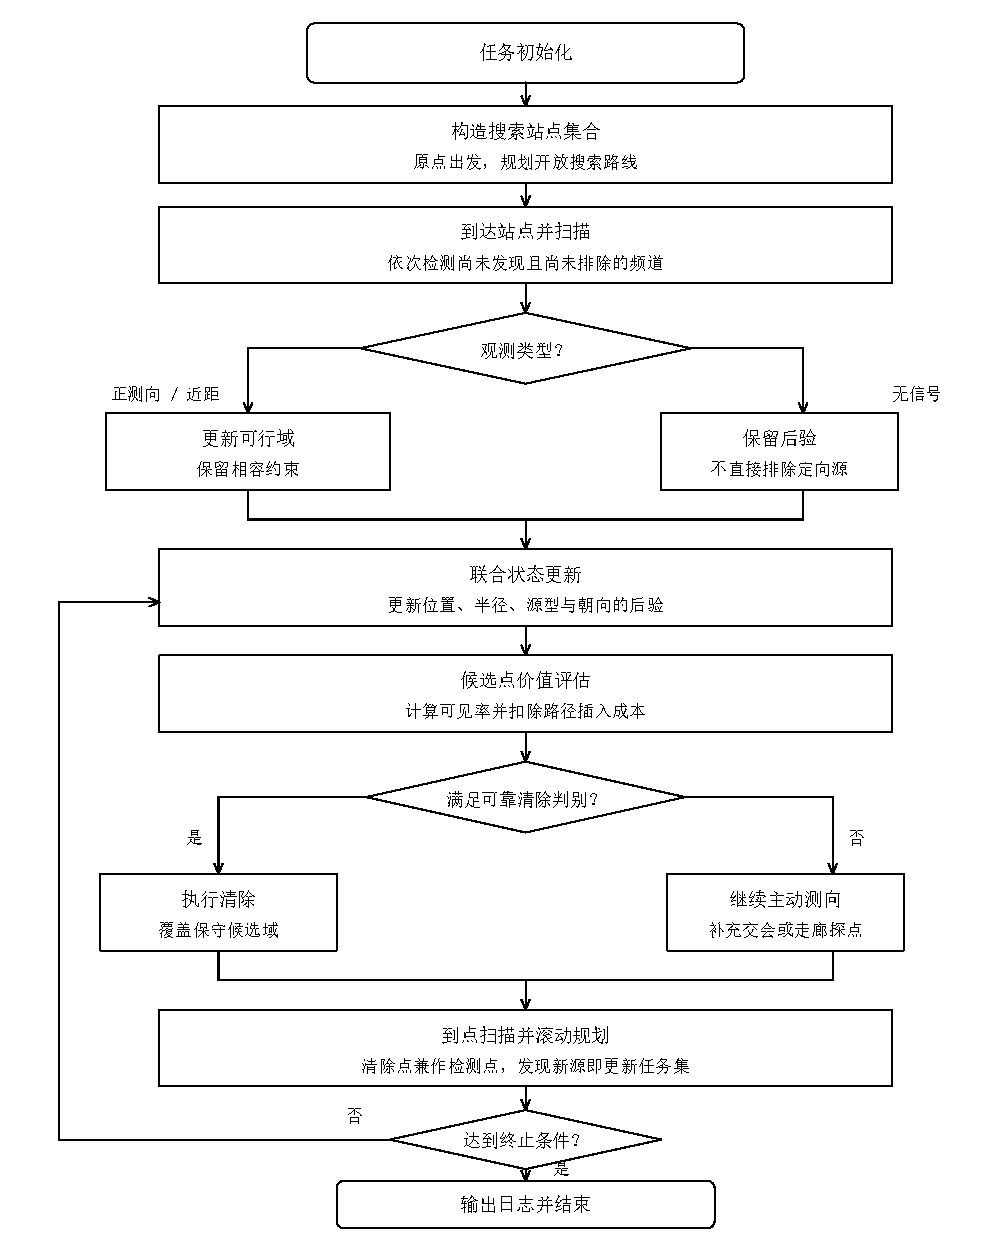
\includegraphics[width=0.88\linewidth]{figures/fig_q4_search_localize_clear_flowchart.pdf}
\caption{问题四搜索、定位与清除的全局闭环流程}
\label{fig:q4-workflow}
\end{figure}

\subsubsection{参数设置与来源}

上述策略涉及的阈值与系数统一列于表\ref{tab:q4_params}。其中 $t_0$ 为单次检测动作的固定耗时，由题设给出；其余均为离线随机场景调参得到的算法参数，而非题设常数，其稳健性将在模型检验部分通过阈值扰动与策略消融加以验证。

\begin{table}[H]
\centering
\caption{问题四关键参数及取值来源}
\label{tab:q4_params}
\begin{tabular}{clll}
\toprule
参数 & 含义 & 取值 & 来源 \\
\midrule
$t_0$ & 单次检测固定时间 & 5 s & 题设 \\
$\alpha_{\min}$ & 快速交会最小夹角 & $12^\circ$ & 离线调参 \\
$\rho_{\rm fast}$ & 快速局部清除最大外包半径 & 120 m & 离线调参 \\
$r_{\rm scout}$ & 分散普查半径 & 800 m & 离线调参 \\
$k_{\rm dense}$ & 高密度场景阈值 & 9 & 离线调参 \\
$B_{\rm probe}$ & 联合探点预算 & 2--4 & 自适应 \\
$L$ & 粒子数量 & $2\times10^5$ & 数值设置 \\
$\lambda$ & 移动惩罚系数 & $4.5\times10^{-4}$ & 离线调参 \\
\bottomrule
\end{tabular}
\end{table}

\subsubsection{正式测试结果与分析}



\begin{table}[H]
\centering
\caption{问题四三次正式测试结果}
\label{tab:q4_official_results}
\begin{tabular}{clccc}
\toprule
测试案例编码 & 清除数 & 虚拟总时间/s & 平均时间/(s/源) & 程序运行时间/s \\
\midrule
\texttt{ARZE-CVT7-NKA3-3W5T} & 11 & 4484.645 & 407.695 & 7.875 \\
\texttt{H75C-SNQU-H5V8-22AR} & 16 & 3118.370 & 194.898 & 8.422 \\
\texttt{6T5H-RU9E-CDEE-JCAF} & 10 & 5086.548 & 508.655 & 7.953 \\
\midrule
合计 & 37 & 12689.563 & 342.961 & -- \\
\bottomrule
\end{tabular}
\end{table}

三次正式测试共获得 $37$ 次成功清除反馈，对应累计虚拟时间 $12689.563$ s；按成功清除源统一加权后，平均定位清除时间为
\[
\bar T_{\rm pooled}=\frac{12689.563}{37}=342.961\ \text{s/源}.
\]
这一合并口径比三次单位时间的简单算术平均 $(407.695+194.898+508.655)/3=370.416$ s/源 更能反映“每个源的平均耗时”。



\section{模型检验与敏感性分析}
围绕输入误差、关键参数和极端情景分别开展检验，并说明结论在何种扰动范围内保持稳定。不能只报告“效果较好”，应给出可复核的量化证据。

\section{模型评价与推广}
可以考虑在第五部分按题目分别展示就行
总结模型的解释性、计算效率、数据依赖和适用边界。推广时明确哪些结构可复用，哪些参数必须重新估计。

% 2026 强制要求：AI 工具使用声明必须置于参考文献之前。
\CumcmAIUsed{问题四论文结构梳理、可视化绘图与文字润色}

\nocite{jiang2003modeling}
\bibliographystyle{gbt7714-numerical}
\bibliography{references}

\appendix
\section{支撑材料文件列表}
支撑材料应单独压缩为 RAR 或 ZIP，且不超过 \SI{20}{MB}。示例清单如下；提交前必须与实际压缩包逐项一致。
\begin{longtable}{@{}p{0.08\textwidth}p{0.34\textwidth}p{0.46\textwidth}@{}}
  \toprule
  序号 & 文件路径 & 内容说明 \\
  \midrule
  1 & \texttt{code/example.py} & 可运行的示例程序 \\
  2 & \texttt{data/processed.csv} & 自主获取并清洗后的数据（示例，按实际替换） \\
  3 & \texttt{AI工具使用详情.pdf} & 仅在使用 AI 工具时提供 \\
  \bottomrule
\end{longtable}

\section{完整源程序}
建模所用的全部源程序必须完整、可运行，并与论文结果一致。此处演示从文件直接载入代码，避免论文附录与支撑材料中的代码版本漂移。
\lstinputlisting[language=Python,basicstyle=\ttfamily\scriptsize,caption={示例程序}]{code/example.py}

\end{document}
